\ifx\type\undefined
  \documentclass[10pt, t]{beamer}
  \setbeamertemplate{footline}[page number]
\else
  \documentclass[10pt]{article}
  \usepackage[margin=1in]{geometry}
\fi

\usepackage{amsmath}
\usepackage{amssymb}
\usepackage{amsthm}
\usepackage{bbm}
\usepackage{cancel}
\usepackage{listings}
\usepackage{mathrsfs}
\usepackage{multirow}
\usepackage{soul}
\usepackage{stmaryrd}
\usepackage{tikz}
\usepackage{tikz-cd}
\usepackage{wrapfig}

\newtheorem*{algorithm}{Algorithm}
\newtheorem*{assumptions}{Assumptions}
\newtheorem*{conjecture}{Conjecture}
\newtheorem*{consequences}{Consequences}
\newtheorem*{exercise}{Exercise}
\newtheorem*{formalisation}{Formalisation}
\newtheorem*{proposition}{Proposition}
\newtheorem*{question}{Question}
\newtheorem*{remark}{Remark}

\ifx\type\undefined\else
  \newtheorem*{definition}{Definition}
  \newtheorem*{example}{Example}
  \newtheorem*{lemma}{Lemma}
  \newtheorem*{theorem}{Theorem}
\fi

\definecolor{keywordcolor}{rgb}{0.7, 0.1, 0.1}
\definecolor{tacticcolor}{rgb}{0.0, 0.1, 0.6}
\definecolor{commentcolor}{rgb}{0.4, 0.4, 0.4}
\definecolor{symbolcolor}{rgb}{0.0, 0.1, 0.6}
\definecolor{sortcolor}{rgb}{0.1, 0.5, 0.1}
\definecolor{attributecolor}{rgb}{0.7, 0.1, 0.1}
\def\lstlanguagefiles{lstlean.tex}
\lstset{language=lean}

\newcommand\A{\mathbb{A}}
\newcommand\C{\mathbb{C}}
\newcommand\F{\mathbb{F}}
\newcommand\G{\mathbb{G}}
\renewcommand\H{\mathbb{H}}
\newcommand\I{\mathbb{I}}
\newcommand\N{\mathbb{N}}
\renewcommand\P{\mathbb{P}}
\newcommand\Q{\mathbb{Q}}
\newcommand\R{\mathbb{R}}
\newcommand\Z{\mathbb{Z}}

\renewcommand\AA{\mathcal{A}}
\newcommand\BB{\mathcal{B}}
\newcommand\CC{\mathcal{C}}
\newcommand\DD{\mathcal{D}}
\newcommand\EE{\mathcal{E}}
\newcommand\FF{\mathcal{F}}
\newcommand\GG{\mathcal{G}}
\newcommand\HH{\mathcal{H}}
\newcommand\II{\mathcal{I}}
\newcommand\LL{\mathcal{L}}
\newcommand\MM{\mathcal{M}}
\newcommand\NN{\mathcal{N}}
\newcommand\OO{\mathcal{O}}
\newcommand\PP{\mathcal{P}}
\newcommand\RR{\mathcal{R}}
\renewcommand\SS{\mathcal{S}}
\newcommand\TT{\mathcal{T}}
\newcommand\XX{\mathcal{X}}

\renewcommand\aa{\mathfrak{a}}
\newcommand\cc{\mathfrak{c}}
\newcommand\dd{\mathfrak{d}}
\newcommand\ff{\mathfrak{f}}
\renewcommand\gg{\mathfrak{g}}
\newcommand\mm{\mathfrak{m}}
\newcommand\pp{\mathfrak{p}}
\newcommand\qq{\mathfrak{q}}
\renewcommand\ss{\mathfrak{s}}

\newcommand\LLL{\mathscr{L}}

\newcommand\ab{\mathrm{ab}}
\newcommand\Ab{\mathbf{Ab}}
\newcommand\Alg{\mathbf{Alg}}
\newcommand\Aff{\mathbf{Aff}}
\newcommand\Aut{\operatorname{Aut}}
\newcommand\Az{\mathrm{Az}}
\newcommand\Br{\operatorname{Br}}
\newcommand\BSD{\operatorname{BSD}}
\newcommand\ch{\operatorname{char}}
\newcommand\Cl{\operatorname{Cl}}
\newcommand\coker{\operatorname{coker}}
\newcommand\cris{\mathrm{cris}}
\renewcommand\d{\mathrm{d}}
\newcommand\Div{\operatorname{Div}}
\newcommand\dR{\mathrm{dR}}
\newcommand\EN{\operatorname{EN}}
\newcommand\End{\operatorname{End}}
\newcommand\ES{\operatorname{ES}}
\newcommand\et{\mathrm{\acute{e}t}}
\newcommand\Et{\mathbf{\acute{E}t}}
\newcommand\Ext{\operatorname{Ext}}
\newcommand\Fr{\operatorname{Fr}}
\newcommand\Frac{\operatorname{Frac}}
\newcommand\Gal{\operatorname{Gal}}
\newcommand\GL{\operatorname{GL}}
\newcommand\Gr{\mathrm{Gr}}
\newcommand\Hom{\operatorname{Hom}}
\newcommand\HT{\mathrm{HT}}
\newcommand\id{\operatorname{id}}
\newcommand\im{\operatorname{im}}
\newcommand\Ind{\operatorname{Ind}}
\renewcommand\inf{\operatorname{inf}}
\newcommand\inv{\operatorname{inv}}
\newcommand\Irr{\operatorname{Irr}}
\newcommand\Jac{\operatorname{Jac}}
\newcommand\lcm{\operatorname{lcm}}
\newcommand\Mat{\operatorname{Mat}}
\newcommand\Mod{\mathbf{Mod}}
\newcommand\Nm{\operatorname{Nm}}
\newcommand\nr{\mathrm{nr}}
\newcommand\NS{\operatorname{NS}}
\newcommand\Ob{\operatorname{Ob}}
\newcommand\ord{\operatorname{ord}}
\newcommand\op{\mathrm{op}}
\newcommand\PGL{\operatorname{PGL}}
\newcommand\Pic{\operatorname{Pic}}
\newcommand\Prob{\operatorname{Prob}}
\newcommand\Proj{\operatorname{Proj}}
\newcommand\PSh{\mathbf{PSh}}
\newcommand\Reg{\operatorname{Reg}}
\newcommand\res{\operatorname{res}}
\newcommand\rk{\operatorname{rk}}
\newcommand\Sch{\mathbf{Sch}}
\newcommand\Sel{\operatorname{Sel}}
\newcommand\Set{\mathbf{Set}}
\newcommand\sgn{\operatorname{sgn}}
\newcommand\Sh{\mathbf{Sh}}
\newcommand\SL{\operatorname{SL}}
\newcommand\Spec{\operatorname{Spec}}
\newcommand\supp{\operatorname{supp}}
\newcommand\Tam{\operatorname{Tam}}
\newcommand\Top{\mathbf{Top}}
\newcommand\tor{\operatorname{tor}}
\newcommand\tr{\operatorname{tr}}
\newcommand\tra{\operatorname{tra}}
\newcommand\WC{\operatorname{WC}}

\DeclareFontFamily{U}{wncyr}{}
\DeclareFontShape{U}{wncyr}{m}{n}{<->wncyr10}{}
\DeclareSymbolFont{cyr}{U}{wncyr}{m}{n}
\DeclareMathSymbol{\Sha}{\mathord}{cyr}{"58}

\newcommand{\function}[5][]{
  \if &#1&
    \begin{array}{rcl}
      #2 & \longrightarrow & #3 \\
      #4 & \longmapsto     & #5
    \end{array}
  \else
    \begin{array}{rcrcl}
      #1 & : & #2 & \longrightarrow & #3 \\
         &   & #4 & \longmapsto     & #5
    \end{array}
  \fi
}

\newcommand{\functions}[7][]{
  \if &#1&
    \begin{array}{rcl}
      #2 & \longrightarrow & #3 \\
      #4 & \longmapsto     & #5 \\
      #6 & \longmapsto     & #7 \\
    \end{array}
  \else
    \begin{array}{rcrcl}
      #1 & : & #2 & \longrightarrow & #3 \\
         &   & #4 & \longmapsto     & #5 \\
         &   & #6 & \longmapsto     & #7
    \end{array}
  \fi
}
\usetheme{singapore}
\usepackage[scheme=plain]{ctex}
\title{Formalising division polynomials in Lean}
\subtitle{Lean 形式化数学学习强化和实践交流研讨会}
\author{David Ang (洪鼎赐)}
\institute{University of East Anglia}
\date{Monday, 26 January 2026}

\begin{document}

\frame\maketitle

\section{Introduction}

\begin{frame}{The weak Birch and Swinnerton-Dyer conjecture}

Let $ E $ be an elliptic curve over a number field $ K $.

\begin{conjecture}[weak Birch and Swinnerton-Dyer]
The rank of $ E $ is the order of vanishing of its L-function $ L(E, s) $ at $ s = 1 $.
\end{conjecture}

\bigskip Here, the \emph{L-function} of $ E $ is given by
$$ L(E, s) := \prod_p \dfrac{1}{L_p(E, s)}, $$
where $ p $ runs over all primes of $ K $, and the Euler factor $ L_p(E, s) $ is defined in terms of the \emph{$ \ell $-adic Galois representation} $ \rho_{E, \ell} $ for any prime $ \ell $ with $ p \nmid \ell $. This is the action of the absolute Galois group of $ K_p $ on the \emph{$ \ell $-adic Tate module} $ T_\ell E $, which is the inverse limit of \emph{$ \ell^n $-torsion subgroups}
$$ E(\overline{K_p})[\ell^n] := \{P \in E(\overline{K_p}) : [\ell^n](P) = 0\}, $$
with respect to the multiplication-by-$ \ell $ maps $ [\ell] : E(\overline{K_p}) \to E(\overline{K_p}) $.

\end{frame}

\begin{frame}{The $ n $-torsion subgroup and the $ \ell $-adic Tate module}

Let $ E $ be an elliptic curve over a perfect field $ F $.

\begin{theorem}[main]
$ \#E(\overline{F})[n] = n^2 $ for any $ n \in \N $ with $ \ch(F) \nmid n $.
\end{theorem}

\bigskip If $ G $ is an abelian group such that $ \#G[n] = n^d $ for all $ n \in \N $, then $ G[n] \cong (\Z / n)^d $ by the structure theorem of finite abelian groups. In particular, $ E(\overline{F})[n] \cong (\Z / n)^2 $ for any $ n \in \N $ with $ \ch(F) \nmid n $, so
$$
\begin{tikzcd}[ampersand replacement=\&]
T_\ell E \arrow{d}{\sim} \&[-30] := \varprojlim\Big(\dots \arrow{r}{[\ell]} \& E(\overline{F})[\ell^3] \arrow{r}{[\ell]} \arrow{d}{\sim} \& E(\overline{F})[\ell^2] \arrow{r}{[\ell]} \arrow{d}{\sim} \& E(\overline{F})[\ell]\Big) \arrow{d}{\sim} \\
\Z_\ell^2 \& := \varprojlim\Big(\dots \arrow{r}{\bmod\ell^3} \& (\Z / \ell^3)^2 \arrow{r}{\bmod\ell^2} \& (\Z / \ell^2)^2 \arrow{r}{\bmod\ell} \& (\Z / \ell)^2\Big).
\end{tikzcd}
$$
吴培然 formalised the reduction of $ \rho_{E, \ell} $ to the main theorem.

\end{frame}

\begin{frame}{An infamous exercise}

\emph{The Arithmetic of Elliptic Curves} by Silverman gives several approaches to the main theorem (see Theorem III.6.4(b) and Theorem VI.6.1(a)).

\begin{exercise}[3.7(d)]
Let $ n \in \Z $. Prove that for any point $ (x, y) \in E(F) $,
$$ [n]((x, y)) = \left(\dfrac{\phi_n(x, y)}{\psi_n(x, y)^2}, \dfrac{\omega_n(x, y)}{\psi_n(x, y)^3}\right). $$
\end{exercise}

Silverman gives definitions for $ \phi_n, \omega_n \in F[X, Y] $ in terms of certain \emph{division polynomials} $ \psi_n \in F[X, Y] $, which feature in Schoof's algorithm.

\bigskip

\begin{conjecture}[洪]
No one has done Exercise 3.7 purely algebraically.
\end{conjecture}

许俊彦 formalised a complete solution to Exercise 3.7(d).

\end{frame}

\section{Definitions}

\begin{frame}{The polynomials $ \psi_n $}

The $ n $-th \textbf{division polynomial} $ \psi_n \in R[X, Y] $ is given by
\begin{align*}
\psi_0 & := 0, \\
\psi_1 & := 1, \\
\psi_2 & := 2Y + a_1X + a_3, \\
\psi_3 & := \bigcirc \\
& \qquad \text{where} \ \bigcirc := 3X^4 + b_2X^3 + 3b_4X^2 + 3b_6X + b_8, \\
\psi_4 & := \psi_2\triangle \\
& \qquad \text{where} \ \triangle := {\scriptscriptstyle 2X^6 + b_2X^5 + 5b_4X^4 + 10b_6X^3 + 10b_8X^2 + (b_2b_8 - b_4b_6)X + (b_4b_8 - b_6^2)}, \\
\psi_{2n + 1} & := \psi_{n + 2}\psi_n^3 - \psi_{n - 1}\psi_{n + 1}^3, \\
\psi_{2n} & := \dfrac{\psi_{n - 1}^2\psi_n\psi_{n + 2} - \psi_{n - 2}\psi_n\psi_{n + 1}^2}{\psi_2}, \\
\psi_{-n} & := -\psi_n.
\end{align*}
In \texttt{mathlib}, $ \psi_n $ is defined in terms of $ \Psi_n \in R[X] $.

\end{frame}

\begin{frame}{The polynomials $ \Psi_n $}

The polynomial $ \Psi_n \in R[X] $ is given by
\begin{align*}
\Psi_0 & := 0, \\
\Psi_1 & := 1, \\
\Psi_2 & := 1, \\
\Psi_3 & := \bigcirc, \\
\Psi_4 & := \triangle, \\
\Psi_{2n + 1} & :=
\begin{cases}
\Psi_{n + 2}\Psi_n^3 - \square^2\Psi_{n - 1}\Psi_{n + 1}^3 & \text{if} \ n \ \text{is odd}, \\
\square^2\Psi_{n + 2}\Psi_n^3 - \Psi_{n - 1}\Psi_{n + 1}^3 & \text{if} \ n \ \text{is even},
\end{cases} \\
& \qquad \text{where} \ \square := 4X^3 + b_2X^2 + 2b_4X + b_6, \\
\Psi_{2n} & := \Psi_{n - 1}^2\Psi_n\Psi_{n + 2} - \Psi_{n - 2}\Psi_n\Psi_{n + 1}^2, \\
\Psi_{-n} & := -\Psi_n.
\end{align*}
Then $ \psi_n = \Psi_n $ when $ n $ is odd and $ \psi_n = \psi_2\Psi_n $ when $ n $ is even.

\end{frame}

\begin{frame}{The polynomials $ \phi_n $ and $ \Phi_n $}

Modulo the Weierstrass equation $ E(X, Y) $ defining $ E $,
\begin{align*}
\psi_2^2
& = (2Y + a_1X + a_3)^2 \\
& = 4(Y^2 + a_1XY + a_3Y) + a_1^2X^2 + 2a_1a_3X + a_3^2 \\
& \equiv \underbrace{4X^3 + b_2X^2 + 2b_4X + b_6}_\square \mod E(X, Y).
\end{align*}
In particular, $ \psi_n^2 $ and $ \psi_{n + 1}\psi_{n - 1} $ are congruent to polynomials in $ R[X] $.

\bigskip The polynomial $ \phi_n \in R[X, Y] $ is given by
$$ \phi_n := X\psi_n^2 - \psi_{n + 1}\psi_{n - 1}, $$
so that $ \phi_n \equiv \Phi_n \mod E(X, Y) $, where $ \Phi_n \in R[X] $ is given by
$$ \Phi_n :=
\begin{cases}
X\Psi_n^2 - \square\Psi_{n + 1}\Psi_{n - 1} & \text{if} \ n \ \text{is odd}, \\
X\square\Psi_n^2 - \Psi_{n + 1}\Psi_{n - 1} & \text{if} \ n \ \text{is even}.
\end{cases}
$$

\end{frame}

\begin{frame}{The polynomials $ \omega_n $}

The polynomial $ \omega_n \in R[X, Y] $ is given by
$$ \omega_n := \dfrac{1}{2}\left(\dfrac{\psi_{2n}}{\psi_n} - a_1\phi_n\psi_n - a_3\psi_n^3\right). $$

\begin{lemma}[许]
Let $ n \in \Z $. Then $ \psi_{2n} / \psi_n - a_1\phi_n\psi_n - a_3\psi_n^3 $ is divisible by $ 2 $ in $ \Z[a_i, X, Y] $.
\end{lemma}

\begin{example}[$ a_1 = a_3 = 0 $]
\vspace{-0.5cm}
$$ \omega_2 = \dfrac{\Psi_4}{2} = \dfrac{\scriptstyle 2X^6 + 4a_2X^5 + 10a_4X^4 + 40a_6X^3 + 10b_8X^2 + (4a_2b_8 - 8a_4a_6)X + (2a_4b_8 - 16a_6^2)}{2}. $$
\end{example}

Define $ \omega_n $ as the image of the quotient under $ \Z[a_i, X, Y] \to R[X, Y] $.

\bigskip When $ n = 4 $, this quotient has 15,049 terms.

\end{frame}

\section{Remarks}

\begin{frame}{Elliptic divisibility sequences and elliptic nets}

Integrality relies on the fact that $ \psi_n $ is an \textbf{elliptic divisibility sequence}.

\begin{exercise}[3.7(g)]
For all $ n, m, r \in \Z $, prove that $ \psi_n \mid \psi_{nm} $ and
$$ \psi_{n + m}\psi_{n - m}\psi_r^2 = \psi_{n + r}\psi_{n - r}\psi_m^2 - \psi_{m + r}\psi_{m - r}\psi_n^2. $$
\end{exercise}

Note that this generalises the recursive definitions of $ \psi_{2n + 1} $ and $ \psi_{2n} $.

\bigskip Surprisingly, this needs the stronger result that $ \psi_n $ is an \textbf{elliptic net}.

\begin{theorem}[许]
Let $ n, m, r, s \in \Z $. Then
$$ \psi_{n + m}\psi_{n - m}\psi_{r + s}\psi_{r - s} = \psi_{n + r}\psi_{n - r}\psi_{m + s}\psi_{m - s} - \psi_{m + r}\psi_{m - r}\psi_{n + s}\psi_{n - s}. $$
\end{theorem}

Elliptic divisibility sequences were first introduced by Morgan Ward (1948) and generalised to elliptic nets by Katherine Stange (2008).

\end{frame}

\begin{frame}{Other formalised results}

The polynomial $ \Psi_n^{(2)} \in R[X] $ is given by
$$ \Psi_n^{(2)} :=
\begin{cases}
\Psi_n^2 & \text{if} \ n \ \text{is odd}, \\
\square\Psi_n^2 & \text{if} \ n \ \text{is even},
\end{cases}
$$
so that $ \Psi_2^{(2)} = \square $ and $ \Psi_n^{(2)} \equiv \psi_n^2 \mod E(X, Y) $.

\bigskip

\begin{exercise}[3.7(b)]
Show that $ \Phi_n = X^{n^2} + \dots $ and $ \Psi_n^{(2)} = n^2X^{n^2 - 1} + \dots $.
\end{exercise}

This is an inductive computation of \texttt{natDegree} and \texttt{leadingCoeff}.

\bigskip

\begin{exercise}[3.7(c)]
Prove that $ \Phi_n $ and $ \Psi_n^{(2)} $ are relatively prime.
\end{exercise}

Surprisingly, this needs Exercise 3.7(d) and the assumption that $ \Delta \ne 0 $.

\end{frame}

\begin{frame}[c]{A blueprint for the $ \ell $-adic Tate module}

\begin{center}
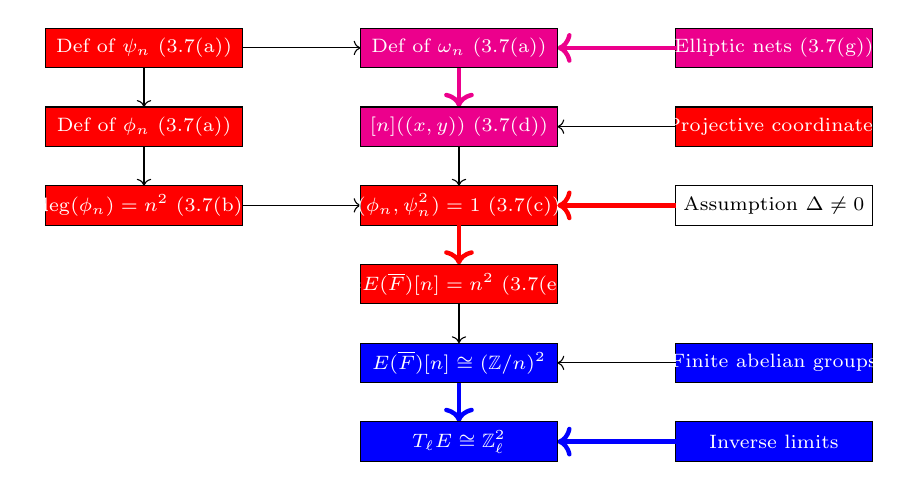
\begin{tikzpicture}
\draw [fill=red] (0, 0) rectangle node[color=white]{\scriptsize Def of $ \psi_n $ (3.7(a))} (2.5, -0.5);
\draw [->] (1.25, -0.5) to (1.25, -1);
\draw [fill=red] (0, -1) rectangle node[color=white]{\scriptsize Def of $ \phi_n $ (3.7(a))} (2.5, -1.5);
\draw [->] (1.25, -1.5) to (1.25, -2);
\draw [fill=red] (0, -2) rectangle node[color=white]{\scriptsize $ \deg(\phi_n) = n^2 $ (3.7(b))} (2.5, -2.5);
\draw [fill=red] (8, -1) rectangle node[color=white]{\scriptsize Projective coordinates} (10.5, -1.5);
\draw [->] (2.5, -0.25) to (4, -0.25);
\draw [fill=magenta] (8, 0) rectangle node[color=white]{\scriptsize Elliptic nets (3.7(g))} (10.5, -0.5);
\draw [->, color=magenta, ultra thick] (8, -0.25) to (6.5, -0.25);
\draw [fill=magenta] (4, 0) rectangle node[color=white]{\scriptsize Def of $ \omega_n $ (3.7(a))} (6.5, -0.5);
\draw [->, color=magenta, ultra thick] (5.25, -0.5) to (5.25, -1);
\draw [->] (8, -1.25) to (6.5, -1.25);
\draw [fill=magenta] (4, -1) rectangle node[color=white]{\scriptsize $ [n]((x, y)) $ (3.7(d))} (6.5, -1.5);
\draw [->] (5.25, -1.5) to (5.25, -2);
\draw [->] (2.5, -2.25) to (4, -2.25);
\draw [fill=red] (4, -2) rectangle node[color=white]{\scriptsize $ (\phi_n, \psi_n^2) = 1 $ (3.7(c))} (6.5, -2.5);
\draw [->, color=red, ultra thick] (5.25, -2.5) to (5.25, -3);
\draw [fill=red] (4, -3) rectangle node[color=white]{\scriptsize $ \#E(\overline{F})[n] = n^2 $ (3.7(e))} (6.5, -3.5);
\draw [->] (5.25, -3.5) to (5.25, -4);
\draw [fill=blue] (8, -4) rectangle node[color=white]{\scriptsize Finite abelian groups} (10.5, -4.5);
\draw [->] (8, -4.25) to (6.5, -4.25);
\draw [fill=blue] (4, -4) rectangle node[color=white]{\scriptsize $ E(\overline{F})[n] \cong (\Z / n)^2 $} (6.5, -4.5);
\draw [->, color=blue, ultra thick] (5.25, -4.5) to (5.25, -5);
\draw [fill=blue] (8, -5) rectangle node[color=white]{\scriptsize Inverse limits} (10.5, -5.5);
\draw [->, color=blue, ultra thick] (8, -5.25) to (6.5, -5.25);
\draw [fill=blue] (4, -5) rectangle node[color=white]{\scriptsize $ T_\ell E \cong \Z_\ell^2 $} (6.5, -5.5);
\draw (8, -2) rectangle node{\scriptsize Assumption $ \Delta \ne 0 $} (10.5, -2.5);
\draw [->, color=red, ultra thick] (8, -2.25) to (6.5, -2.25);
\end{tikzpicture}
\end{center}

\end{frame}

\end{document}